% Options for packages loaded elsewhere
\PassOptionsToPackage{unicode}{hyperref}
\PassOptionsToPackage{hyphens}{url}
%
\documentclass[
  ignorenonframetext,
]{beamer}
\usepackage{pgfpages}
\setbeamertemplate{caption}[numbered]
\setbeamertemplate{caption label separator}{: }
\setbeamercolor{caption name}{fg=normal text.fg}
\beamertemplatenavigationsymbolsempty
% Prevent slide breaks in the middle of a paragraph
\widowpenalties 1 10000
\raggedbottom
\setbeamertemplate{part page}{
  \centering
  \begin{beamercolorbox}[sep=16pt,center]{part title}
    \usebeamerfont{part title}\insertpart\par
  \end{beamercolorbox}
}
\setbeamertemplate{section page}{
  \centering
  \begin{beamercolorbox}[sep=12pt,center]{part title}
    \usebeamerfont{section title}\insertsection\par
  \end{beamercolorbox}
}
\setbeamertemplate{subsection page}{
  \centering
  \begin{beamercolorbox}[sep=8pt,center]{part title}
    \usebeamerfont{subsection title}\insertsubsection\par
  \end{beamercolorbox}
}
\AtBeginPart{
  \frame{\partpage}
}
\AtBeginSection{
  \ifbibliography
  \else
    \frame{\sectionpage}
  \fi
}
\AtBeginSubsection{
  \frame{\subsectionpage}
}
\usepackage{lmodern}
\usepackage{amssymb,amsmath}
\usepackage{ifxetex,ifluatex}
\ifnum 0\ifxetex 1\fi\ifluatex 1\fi=0 % if pdftex
  \usepackage[T1]{fontenc}
  \usepackage[utf8]{inputenc}
  \usepackage{textcomp} % provide euro and other symbols
\else % if luatex or xetex
  \usepackage{unicode-math}
  \defaultfontfeatures{Scale=MatchLowercase}
  \defaultfontfeatures[\rmfamily]{Ligatures=TeX,Scale=1}
\fi
\usetheme[]{CambridgeUS}
\usecolortheme{dolphin}
\usefonttheme{structurebold}
% Use upquote if available, for straight quotes in verbatim environments
\IfFileExists{upquote.sty}{\usepackage{upquote}}{}
\IfFileExists{microtype.sty}{% use microtype if available
  \usepackage[]{microtype}
  \UseMicrotypeSet[protrusion]{basicmath} % disable protrusion for tt fonts
}{}
\makeatletter
\@ifundefined{KOMAClassName}{% if non-KOMA class
  \IfFileExists{parskip.sty}{%
    \usepackage{parskip}
  }{% else
    \setlength{\parindent}{0pt}
    \setlength{\parskip}{6pt plus 2pt minus 1pt}}
}{% if KOMA class
  \KOMAoptions{parskip=half}}
\makeatother
\usepackage{xcolor}
\IfFileExists{xurl.sty}{\usepackage{xurl}}{} % add URL line breaks if available
\IfFileExists{bookmark.sty}{\usepackage{bookmark}}{\usepackage{hyperref}}
\hypersetup{
  pdftitle={Introduction to R programming language},
  pdfauthor={Ezekiel Adebayo Ogundepo},
  hidelinks,
  pdfcreator={LaTeX via pandoc}}
\urlstyle{same} % disable monospaced font for URLs
\newif\ifbibliography
\usepackage{color}
\usepackage{fancyvrb}
\newcommand{\VerbBar}{|}
\newcommand{\VERB}{\Verb[commandchars=\\\{\}]}
\DefineVerbatimEnvironment{Highlighting}{Verbatim}{commandchars=\\\{\}}
% Add ',fontsize=\small' for more characters per line
\usepackage{framed}
\definecolor{shadecolor}{RGB}{248,248,248}
\newenvironment{Shaded}{\begin{snugshade}}{\end{snugshade}}
\newcommand{\AlertTok}[1]{\textcolor[rgb]{0.94,0.16,0.16}{#1}}
\newcommand{\AnnotationTok}[1]{\textcolor[rgb]{0.56,0.35,0.01}{\textbf{\textit{#1}}}}
\newcommand{\AttributeTok}[1]{\textcolor[rgb]{0.77,0.63,0.00}{#1}}
\newcommand{\BaseNTok}[1]{\textcolor[rgb]{0.00,0.00,0.81}{#1}}
\newcommand{\BuiltInTok}[1]{#1}
\newcommand{\CharTok}[1]{\textcolor[rgb]{0.31,0.60,0.02}{#1}}
\newcommand{\CommentTok}[1]{\textcolor[rgb]{0.56,0.35,0.01}{\textit{#1}}}
\newcommand{\CommentVarTok}[1]{\textcolor[rgb]{0.56,0.35,0.01}{\textbf{\textit{#1}}}}
\newcommand{\ConstantTok}[1]{\textcolor[rgb]{0.00,0.00,0.00}{#1}}
\newcommand{\ControlFlowTok}[1]{\textcolor[rgb]{0.13,0.29,0.53}{\textbf{#1}}}
\newcommand{\DataTypeTok}[1]{\textcolor[rgb]{0.13,0.29,0.53}{#1}}
\newcommand{\DecValTok}[1]{\textcolor[rgb]{0.00,0.00,0.81}{#1}}
\newcommand{\DocumentationTok}[1]{\textcolor[rgb]{0.56,0.35,0.01}{\textbf{\textit{#1}}}}
\newcommand{\ErrorTok}[1]{\textcolor[rgb]{0.64,0.00,0.00}{\textbf{#1}}}
\newcommand{\ExtensionTok}[1]{#1}
\newcommand{\FloatTok}[1]{\textcolor[rgb]{0.00,0.00,0.81}{#1}}
\newcommand{\FunctionTok}[1]{\textcolor[rgb]{0.00,0.00,0.00}{#1}}
\newcommand{\ImportTok}[1]{#1}
\newcommand{\InformationTok}[1]{\textcolor[rgb]{0.56,0.35,0.01}{\textbf{\textit{#1}}}}
\newcommand{\KeywordTok}[1]{\textcolor[rgb]{0.13,0.29,0.53}{\textbf{#1}}}
\newcommand{\NormalTok}[1]{#1}
\newcommand{\OperatorTok}[1]{\textcolor[rgb]{0.81,0.36,0.00}{\textbf{#1}}}
\newcommand{\OtherTok}[1]{\textcolor[rgb]{0.56,0.35,0.01}{#1}}
\newcommand{\PreprocessorTok}[1]{\textcolor[rgb]{0.56,0.35,0.01}{\textit{#1}}}
\newcommand{\RegionMarkerTok}[1]{#1}
\newcommand{\SpecialCharTok}[1]{\textcolor[rgb]{0.00,0.00,0.00}{#1}}
\newcommand{\SpecialStringTok}[1]{\textcolor[rgb]{0.31,0.60,0.02}{#1}}
\newcommand{\StringTok}[1]{\textcolor[rgb]{0.31,0.60,0.02}{#1}}
\newcommand{\VariableTok}[1]{\textcolor[rgb]{0.00,0.00,0.00}{#1}}
\newcommand{\VerbatimStringTok}[1]{\textcolor[rgb]{0.31,0.60,0.02}{#1}}
\newcommand{\WarningTok}[1]{\textcolor[rgb]{0.56,0.35,0.01}{\textbf{\textit{#1}}}}
\usepackage{longtable,booktabs}
\usepackage{caption}
% Make caption package work with longtable
\makeatletter
\def\fnum@table{\tablename~\thetable}
\makeatother
\usepackage{graphicx,grffile}
\makeatletter
\def\maxwidth{\ifdim\Gin@nat@width>\linewidth\linewidth\else\Gin@nat@width\fi}
\def\maxheight{\ifdim\Gin@nat@height>\textheight\textheight\else\Gin@nat@height\fi}
\makeatother
% Scale images if necessary, so that they will not overflow the page
% margins by default, and it is still possible to overwrite the defaults
% using explicit options in \includegraphics[width, height, ...]{}
\setkeys{Gin}{width=\maxwidth,height=\maxheight,keepaspectratio}
% Set default figure placement to htbp
\makeatletter
\def\fps@figure{htbp}
\makeatother
\setlength{\emergencystretch}{3em} % prevent overfull lines
\providecommand{\tightlist}{%
  \setlength{\itemsep}{0pt}\setlength{\parskip}{0pt}}
\setcounter{secnumdepth}{-\maxdimen} % remove section numbering

\title{Introduction to R programming language}
\author{Ezekiel Adebayo Ogundepo}
\date{September 28, 2019}
\titlegraphic{\hspace*{8.5cm}
\includegraphics[width=7cm, height=2cm]{Images/Logo.JPG}}

\begin{document}
\frame{\titlepage}

\begin{frame}
  \tableofcontents[hideallsubsections]
\end{frame}
\begin{frame}

\begin{center}
\textbf{Relax, programming in R is cool!}
\end{center}

If you doubt me, please kindly ask Hadley Wickham, Ezekiel
(\href{https://twitter.com/gbganalyst}{@gbganalyst}) and Obisesan
(@obadairo1).

\end{frame}
\section{R for Data Science}


\begin{frame}{R for Data Science}
\protect\hypertarget{r-for-data-science}{}

Data science is an exciting discipline that allows you to turn raw data
into understanding, insight, and knowledge \cite{P}. The goal of R for
Data Science is to help you learn the most important tools in R that
will allow you to do data science. Data science is a huge field, and
there's no way you can master it by reading a single book \cite{P}.

\end{frame}

\begin{frame}{What you will learn}
\protect\hypertarget{what-you-will-learn}{}

\begin{figure}
\centering
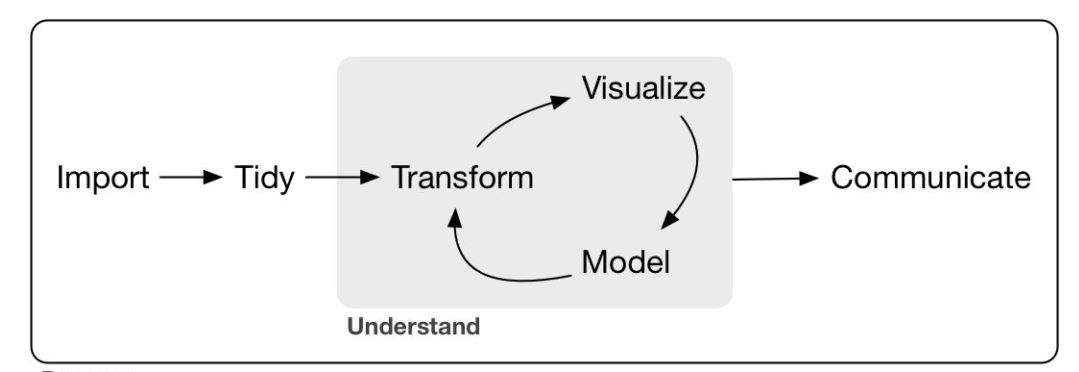
\includegraphics{Images/Capture.JPG}
\caption{Program \textasciitilde{} Inspired by Hadley Wickham \cite{P}}
\end{figure}
\end{frame}


\begin{frame}{What is R programming?}

R is a statistical programming language for data cleaning, analysis, and visualization
\begin{figure}
	\centering
	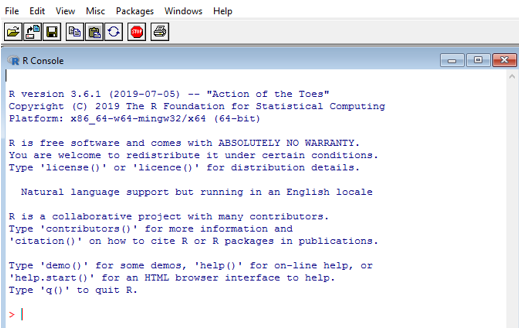
\includegraphics[height=5.8cm, width=13cm]{Images/R.png}
	\caption{R programming}
\end{figure}

\end{frame}


\begin{frame}{What about RStudio?}
	\protect\hypertarget{what-about-rstudio}{}

	R Studio is an integrated development environment (IDE) for R
	programming. R Studio makes programming easier and friendly in R.
	
	\begin{figure}
		\centering
		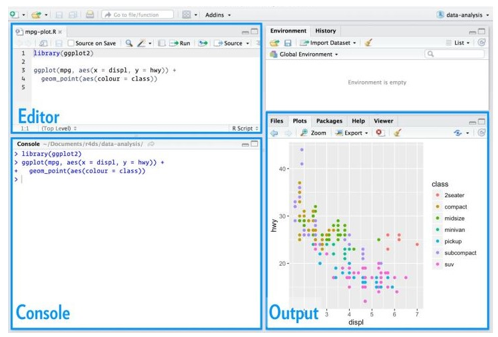
\includegraphics[height=6.5cm, width= 12cm]{Images/R_studio.PNG}
		\caption{R studio}
	\end{figure}
	
\end{frame}

\begin{frame}{R worth it}
\protect\hypertarget{r-worth-it}{}

\begin{figure}
\centering

\includegraphics[width = 18cm, height = 7cm]{Images/r_ladies.JPG}
\caption{R Ladies}
\end{figure}

\end{frame}

\begin{frame}{Introduction to R}
\protect\hypertarget{introduction-to-r}{}

In this section, you will take your first steps with R. You will learn
how to use the console as a calculator and how to assign variables. You
will also get to know the basic data types in R. Let's get started!

\end{frame}

\section{R as a calculator}
\begin{frame}[fragile]{R as a calculator}
\protect\hypertarget{r-as-a-calculator}{}

In its most basic form, R can be used as a simple calculator. Consider
the following arithmetic operations:

\begin{itemize}
\tightlist
\item
  Addition 
\item
  Subtraction 
\item
  Multiplication 
\item
  Division 
\item
  Exponentiation
\item
  Modulo 
\end{itemize}

Calculate \(6 + 12\)

\begin{Shaded}
\begin{Highlighting}[]
\DecValTok{6} \OperatorTok{+}\StringTok{ }\DecValTok{12}
\end{Highlighting}
\end{Shaded}

\begin{verbatim}
## [1] 18
\end{verbatim}

Calculate \(800-900\)

\begin{Shaded}
\begin{Highlighting}[]
\DecValTok{800} \OperatorTok{-}\StringTok{ }\DecValTok{900}
\end{Highlighting}
\end{Shaded}

\begin{verbatim}
## [1] -100
\end{verbatim}

\end{frame}

\begin{frame}[fragile]{R as a calculator}
\protect\hypertarget{r-as-a-calculator-1}{}

Calculate \(4\times 5\)

\begin{Shaded}
\begin{Highlighting}[]
\DecValTok{4} \OperatorTok{*}\StringTok{ }\DecValTok{5}
\end{Highlighting}
\end{Shaded}

\begin{verbatim}
## [1] 20
\end{verbatim}

Calculate \(\frac{2018}{2}\)

\begin{Shaded}
\begin{Highlighting}[]
\DecValTok{2018} \OperatorTok{/}\StringTok{ }\DecValTok{2}
\end{Highlighting}
\end{Shaded}

\begin{verbatim}
## [1] 1009
\end{verbatim}

Calculate \(2^3\)

\begin{Shaded}
\begin{Highlighting}[]
\DecValTok{2}\OperatorTok{^}\DecValTok{3}
\end{Highlighting}
\end{Shaded}

\begin{verbatim}
## [1] 8
\end{verbatim}

\end{frame}

\begin{frame}[fragile]{R as a calculator}
\protect\hypertarget{r-as-a-calculator-2}{}

Calculate \(20\%\%3\)

\begin{Shaded}
\begin{Highlighting}[]
\DecValTok{20} \OperatorTok\StringTok{ }\DecValTok{3}
\end{Highlighting}
\end{Shaded}

\begin{verbatim}
## [1] 2
\end{verbatim}

Calculate the square root of \(\sqrt{4}\)

\begin{Shaded}
\begin{Highlighting}[]
\KeywordTok{sqrt}\NormalTok{(}\DecValTok{4}\NormalTok{)}
\end{Highlighting}
\end{Shaded}

\begin{verbatim}
## [1] 2
\end{verbatim}

Calculate \((\sqrt{4})^2\)

\begin{Shaded}
\begin{Highlighting}[]
\NormalTok{(}\KeywordTok{sqrt}\NormalTok{(}\DecValTok{4}\NormalTok{))}\OperatorTok{^}\DecValTok{2}
\end{Highlighting}
\end{Shaded}

\begin{verbatim}
## [1] 4
\end{verbatim}

\end{frame}

\begin{frame}[fragile]{Comment in R}
\protect\hypertarget{comment-in-r}{}

R makes use of the \# sign to add comments, so that you and others can
understand what the R code is about. Just like Twitter! Comments are not
run as R code, so they will not influence your result. For example, any
code like \(\#3 + 4\) at the console is a comment. R ignores any code in
\#, this means that the code will not run.

\begin{Shaded}
\begin{Highlighting}[]
\CommentTok{# 3+4}
\end{Highlighting}
\end{Shaded}

\end{frame}

\section{Variable and Assignment}
\begin{frame}[fragile]{Variable assignment}
\protect\hypertarget{variable-assignment}{}

A basic concept in \textbf{statistical} programming is called a
variable. A variable allows you to store a value (e.g.~5) or an object
(e.g.~a function description) in R. You can then later use this
variable's name to easily access the value or the object that is stored
with this variable.

\begin{block}{Example}

Store the value of 4 as your first name

\begin{Shaded}
\begin{Highlighting}[]
\NormalTok{ezekiel <-}\StringTok{ }\DecValTok{4}
\end{Highlighting}
\end{Shaded}

To know what is stored in memory as your first name, type your first
name in the console and press return key from the keyboard

\begin{Shaded}
\begin{Highlighting}[]
\NormalTok{ezekiel}
\end{Highlighting}
\end{Shaded}

\begin{verbatim}
## [1] 4
\end{verbatim}

\end{block}

\end{frame}

\begin{frame}[fragile]{Variable assignment and data types in R}
\protect\hypertarget{variable-assignment-and-data-types-in-r}{}

\begin{Shaded}
\begin{Highlighting}[]
\NormalTok{x <-}\StringTok{ }\DecValTok{3}
\NormalTok{y <-}\StringTok{ }\DecValTok{4}
\NormalTok{z <-}\StringTok{ }\DecValTok{10}

\NormalTok{x }\OperatorTok{+}\StringTok{ }\NormalTok{y}
\end{Highlighting}
\end{Shaded}

\begin{verbatim}
## [1] 7
\end{verbatim}

\begin{Shaded}
\begin{Highlighting}[]
\NormalTok{z }\OperatorTok{-}\StringTok{ }\NormalTok{x }\OperatorTok{-}\StringTok{ }\NormalTok{y}
\end{Highlighting}
\end{Shaded}

\begin{verbatim}
## [1] 3
\end{verbatim}

\begin{Shaded}
\begin{Highlighting}[]
\NormalTok{x }\OperatorTok{*}\StringTok{ }\NormalTok{y}
\end{Highlighting}
\end{Shaded}

\begin{verbatim}
## [1] 12
\end{verbatim}

\begin{Shaded}
\begin{Highlighting}[]
\NormalTok{z}\OperatorTok{^}\NormalTok{x}
\end{Highlighting}
\end{Shaded}

\begin{verbatim}
## [1] 1000
\end{verbatim}

\end{frame}

\begin{frame}{Naming Rules for Variables}
\protect\hypertarget{naming-rules-for-variables}{}

The best naming convention is to choose a variable name that will tell
the reader of the program what the variable represents

\begin{block}{Rules for naming variables}

\begin{itemize}
\tightlist
\item
  All variables must begin with a letter of the alphabet.
\item
  After the initial letter, variable names can also contain (\_ or .)
  and numbers. No spaces or special characters, however are allowed.
\item
  Uppercase characters are different from lowercase characters (in R and
  also in Python)
\end{itemize}

\end{block}

\begin{block}{Example}

\begin{table}[ht]
\centering
\begin{tabular}{rll}
  \hline
& Samples of acceptable variable names & Uncceptable variable names \\ 
  \hline
1 & Grade & Grade(Test) \\ 
  2 & test\_grade & test grade \\ 
  3 & term2 & 2 term \\ 
  4 & sales\_price\_2017 & 2017sales\_price \\ 
   \hline
\end{tabular}
\end{table}

\end{block}

\end{frame}

\begin{frame}{Basic classes of objects}
\protect\hypertarget{basic-classes-of-objects}{}

R works with numerous \textbf{atomic} classes of objects. Some of the
most basic atomic data types to get started are:

\begin{itemize}
\tightlist
\item
  Decimas values like 4.7 are called \textbf{numeric}
\item
  Natural numbers like 4 are called \textbf{integers}. Integers are also
  numeric
\item
  Boolean values (\textbf{TRUE} or \textbf{FALSE}) are called
  \textbf{logical}
\item
  Text (or string) values are called \textbf{characters}
\item
  Factors : Categorical variable where each level is a category
\end{itemize}

\end{frame}

\section{Basic data structure in R}
\begin{frame}{Basic data structure or types}
\protect\hypertarget{basic-data-structure-or-types}{}

\begin{enumerate}
\tightlist
\item
  Vector: A collection of elements of the same class
\item
  Matrix: All columns must uniformly contain only one variable type
\item
  data.frame: The columns can contain different classes
\item
  List: Can hold object of different classes and lenght
\end{enumerate}

\end{frame}
\subsection{Vector}
\begin{frame}{Create a vector}
\protect\hypertarget{create-a-vector}{}

Vectors are one-dimensional arrays that can hold numeric data, character
data, or logical data. In R, you can create a vector with the combine
function \textbf{c()}. You place the vector elements separate by a comma
between the parenthesis.

\begin{block}{For example}

numeric\_vector \textless- c(1, 2, 3, 6, 7, 10)

character.vector \textless- c(`Imole', `Emmanuel', `Abono',
`Oresanya', `Ebunlomo')

\end{block}

\begin{block}{Notice}

Adding a space behind the commas in the \textbf{c()} function improves
the readability of your code

\end{block}

\end{frame}

\begin{frame}{Naming a vector}
\protect\hypertarget{naming-a-vector}{}

As a data analyst, it is important to have a clear view on the data that
you are using. Understanding what each element refers to is essential.
You can give a name to the elements of a vector with the
\textbf{names ()} function

\end{frame}

\begin{frame}[fragile]{Create a vector}
\protect\hypertarget{create-a-vector-1}{}

\begin{block}{Example}

\begin{Shaded}
\begin{Highlighting}[]
\NormalTok{sales_tax <-}\StringTok{ }\KeywordTok{c}\NormalTok{(}\DecValTok{140000}\NormalTok{, }\DecValTok{200000}\NormalTok{, }\DecValTok{600000}\NormalTok{, }\DecValTok{180000}\NormalTok{, }\DecValTok{170000}\NormalTok{)}
\KeywordTok{names}\NormalTok{(sales_tax) <-}\StringTok{ }\KeywordTok{c}\NormalTok{(}
  \StringTok{"Monday"}\NormalTok{, }\StringTok{"Tuesday"}\NormalTok{, }\StringTok{"Wednessday"}\NormalTok{,}
  \StringTok{"Thursday"}\NormalTok{, }\StringTok{"Friday"}
\NormalTok{)}
\NormalTok{sales_tax}
\end{Highlighting}
\end{Shaded}

\begin{verbatim}
##     Monday    Tuesday Wednessday   Thursday     Friday 
##     140000     200000     600000     180000     170000
\end{verbatim}

\end{block}

\end{frame}

\begin{frame}[fragile]{Arithmetic with vectors}
\protect\hypertarget{arithmetic-with-vectors}{}

It is important to know that if you sum two vectors in R, it takes the
element-wise sum

\begin{block}{Example}

\begin{Shaded}
\begin{Highlighting}[]
\NormalTok{a <-}\StringTok{ }\KeywordTok{c}\NormalTok{(}\DecValTok{1}\NormalTok{, }\DecValTok{2}\NormalTok{, }\DecValTok{3}\NormalTok{, }\DecValTok{4}\NormalTok{, }\DecValTok{5}\NormalTok{)}
\NormalTok{b <-}\StringTok{ }\KeywordTok{c}\NormalTok{(}\DecValTok{6}\NormalTok{, }\DecValTok{7}\NormalTok{, }\DecValTok{8}\NormalTok{, }\DecValTok{9}\NormalTok{, }\DecValTok{10}\NormalTok{)}
\NormalTok{c <-}\StringTok{ }\NormalTok{a }\OperatorTok{+}\StringTok{ }\NormalTok{b}
\end{Highlighting}
\end{Shaded}

\begin{Shaded}
\begin{Highlighting}[]
\NormalTok{c}
\end{Highlighting}
\end{Shaded}

\begin{verbatim}
## [1]  7  9 11 13 15
\end{verbatim}

\end{block}

\end{frame}

\begin{frame}[fragile]{Vector selection}
\protect\hypertarget{vector-selection}{}

To select elements of a vector (and later matrices, data frames), you
can use square brackets \protect\hyperlink{section}{}, between the
square brackets, you indicate what elements to select.

To select the first elements of vector \textbf{a}, you type
\textbf{a}{[}1{]}.

To select the second element of the vector, you typed \textbf{a}{[}2{]},
etc.

\begin{block}{Example}

\begin{Shaded}
\begin{Highlighting}[]
\NormalTok{a}
\NormalTok{a[}\DecValTok{1}\NormalTok{]}
\NormalTok{a[}\DecValTok{2}\NormalTok{]}
\end{Highlighting}
\end{Shaded}

\end{block}

\end{frame}

\begin{frame}[fragile]{Short group work}
\protect\hypertarget{short-group-work}{}

\begin{block}{What does it do?}

a{[}a\textgreater3{]}

\end{block}

\begin{block}{Create special vectors}

\begin{Shaded}
\begin{Highlighting}[]
\NormalTok{a <-}\StringTok{ }\DecValTok{1}\OperatorTok{:}\DecValTok{10} \CommentTok{# Create sequence 1 to 10}
\NormalTok{b <-}\StringTok{ }\DecValTok{10}\OperatorTok{:}\DecValTok{1} \CommentTok{# Create sequence 10 to 1}
\end{Highlighting}
\end{Shaded}

To create sequence with increament of 2 from 1 to 16, we can
\textbf{seq()} function e.g.

\begin{Shaded}
\begin{Highlighting}[]
\KeywordTok{seq}\NormalTok{(}\DecValTok{1}\NormalTok{, }\DecValTok{16}\NormalTok{, }\DecValTok{2}\NormalTok{)}
\KeywordTok{seq}\NormalTok{(}\DecValTok{1}\NormalTok{, }\DecValTok{20}\NormalTok{, }\FloatTok{0.1}\NormalTok{)}
\KeywordTok{seq}\NormalTok{(}\DecValTok{20}\NormalTok{, }\DecValTok{1}\NormalTok{, }\FloatTok{-0.1}\NormalTok{)}
\end{Highlighting}
\end{Shaded}

\end{block}

\end{frame}

\begin{frame}[fragile]{Create special vectors cont.}
\protect\hypertarget{create-special-vectors-cont.}{}

If you have a sequence value you don't know the last element, say you
just know the start of the sequence and the length of the sequence, e.g.

\begin{Shaded}
\begin{Highlighting}[]
\KeywordTok{seq}\NormalTok{(}\DecValTok{5}\NormalTok{, }\DataTypeTok{by =} \DecValTok{2}\NormalTok{, }\DataTypeTok{length =} \DecValTok{50}\NormalTok{)}
\KeywordTok{length}\NormalTok{(}\KeywordTok{seq}\NormalTok{(}\DecValTok{5}\NormalTok{, }\DataTypeTok{by =} \DecValTok{2}\NormalTok{, }\DataTypeTok{length =} \DecValTok{50}\NormalTok{))}
\end{Highlighting}
\end{Shaded}

Repeating elements for certain number of time

\begin{Shaded}
\begin{Highlighting}[]
\KeywordTok{rep}\NormalTok{(}\DecValTok{5}\NormalTok{, }\DecValTok{10}\NormalTok{) }\CommentTok{# Repeat 5 in 10 times}
\KeywordTok{rep}\NormalTok{(}\DecValTok{1}\OperatorTok{:}\DecValTok{4}\NormalTok{, }\DecValTok{5}\NormalTok{) }\CommentTok{# Repeat 1 to 4 five times}
\KeywordTok{rep}\NormalTok{(}\DecValTok{1}\OperatorTok{:}\DecValTok{4}\NormalTok{, }\DataTypeTok{each =} \DecValTok{3}\NormalTok{) }\CommentTok{# Each element of 1 to 4 3 times}
\end{Highlighting}
\end{Shaded}

\end{frame}

\begin{frame}[fragile]{Short group work}
\protect\hypertarget{short-group-work-1}{}

\begin{block}{Tell us what the following line of codes is or are doing}

\begin{Shaded}
\begin{Highlighting}[]
\KeywordTok{rep}\NormalTok{(}\DecValTok{1}\OperatorTok{:}\DecValTok{4}\NormalTok{, }\DataTypeTok{each =} \DecValTok{3}\NormalTok{, }\DataTypeTok{time =} \DecValTok{2}\NormalTok{)}
\KeywordTok{rep}\NormalTok{(}\DecValTok{1}\OperatorTok{:}\DecValTok{4}\NormalTok{, }\DecValTok{1}\OperatorTok{:}\DecValTok{4}\NormalTok{)}
\KeywordTok{rep}\NormalTok{(}\DecValTok{1}\OperatorTok{:}\DecValTok{4}\NormalTok{, }\KeywordTok{c}\NormalTok{(}\DecValTok{4}\NormalTok{, }\DecValTok{1}\NormalTok{, }\DecValTok{8}\NormalTok{, }\DecValTok{2}\NormalTok{))}
\end{Highlighting}
\end{Shaded}

\end{block}

\end{frame}

\begin{frame}{Group work}
\protect\hypertarget{group-work}{}

\begin{figure}
\centering
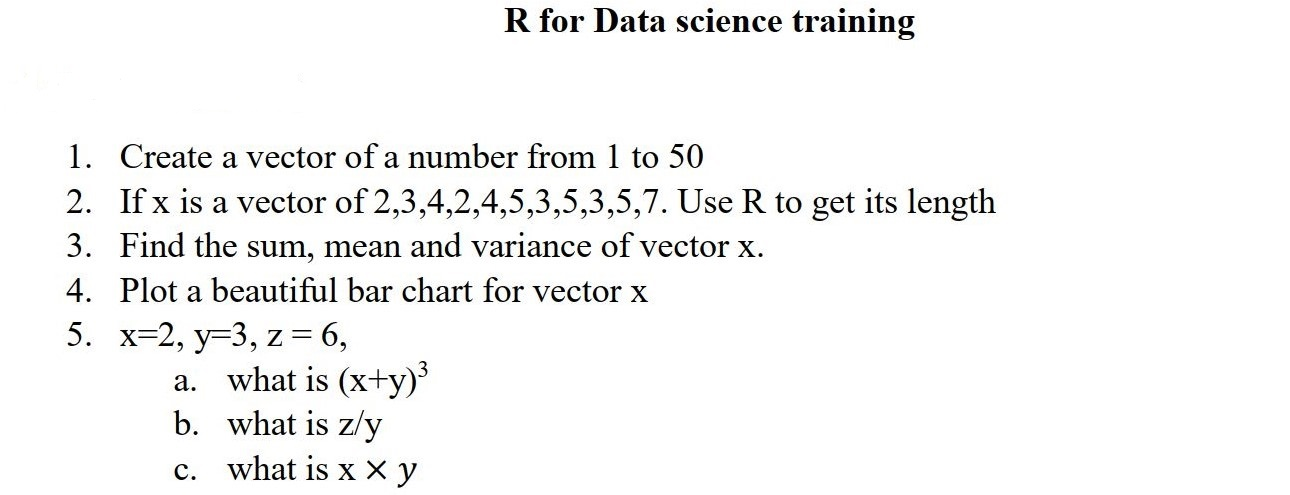
\includegraphics{Images/assignment_Capture.JPG}
\caption{Group work}
\end{figure}

\end{frame}


\subsection{Matrices}

\begin{frame}[fragile]{Matrices}
\protect\hypertarget{matrices}{}

In R, a matrix is a collection of elements of the same data type
(numeric, character, or logical) arranged into a fixed number of rows
and columns.

Since we are only working with rows and columns, a matrix is called two
dimensional array.

You can construct a matrix in R with the \textbf{matrix ()} function.

\begin{block}{Example}

\begin{Shaded}
\begin{Highlighting}[]
\NormalTok{A <-}\StringTok{ }\KeywordTok{matrix}\NormalTok{(}\DecValTok{1}\OperatorTok{:}\DecValTok{9}\NormalTok{, }\DataTypeTok{nrow =} \DecValTok{3}\NormalTok{, }\DataTypeTok{byrow =}\NormalTok{ T)}
\NormalTok{A}
\CommentTok{##      [,1] [,2] [,3]}
\CommentTok{## [1,]    1    2    3}
\CommentTok{## [2,]    4    5    6}
\CommentTok{## [3,]    7    8    9}
\end{Highlighting}
\end{Shaded}

\end{block}

\end{frame}

\begin{frame}{Matrices}
\protect\hypertarget{matrices-1}{}

\begin{itemize}
\tightlist
\item
  The first argument is the collection of elements that \#Rstats will
  arrange into the rows and columns of the matrix. Here, we use 1:9
  which is a shortcut for c(1, 2, \ldots, 9).
\item
  The arguement \textbf{byrow} indicates that the matrix is filled by
  the rows. If we want the matrix to be filled by the columns, we just
  place \textbf{byrow=F}
\item
  The argument \textbf{nrow} indicates that the matrix should have 3
  \textbf{rows}
\end{itemize}

\end{frame}

\begin{frame}{Short group work}
\protect\hypertarget{short-group-work-2}{}

Construct a matrix with 3 rows containing the numbers 1 up to 9 filled
\textbf{column-wise}

\end{frame}

\begin{frame}[fragile]{Progressing from vector to matrix}
\protect\hypertarget{progressing-from-vector-to-matrix}{}

\begin{Shaded}
\begin{Highlighting}[]
\NormalTok{fiscal_year2016_}\DecValTok{17}\NormalTok{ <-}\StringTok{ }\KeywordTok{c}\NormalTok{(}\DecValTok{140}\NormalTok{, }\DecValTok{134}\NormalTok{)}

\NormalTok{fiscal_year2017_}\DecValTok{18}\NormalTok{ <-}\StringTok{ }\KeywordTok{c}\NormalTok{(}\DecValTok{160}\NormalTok{, }\DecValTok{158}\NormalTok{)}

\NormalTok{performance_analysis <-}\StringTok{ }\KeywordTok{matrix}\NormalTok{(}\KeywordTok{c}\NormalTok{(}
\NormalTok{  fiscal_year2016_}\DecValTok{17}\NormalTok{,}
\NormalTok{  fiscal_year2017_}\DecValTok{18}
\NormalTok{),}
\DataTypeTok{nrow =} \DecValTok{2}\NormalTok{,}
\DataTypeTok{ncol =} \DecValTok{2}\NormalTok{, }\DataTypeTok{byrow =}\NormalTok{ T}
\NormalTok{)}
\NormalTok{performance_analysis}
\end{Highlighting}
\end{Shaded}

\begin{verbatim}
##      [,1] [,2]
## [1,]  140  134
## [2,]  160  158
\end{verbatim}

\end{frame}

\begin{frame}[fragile]{Naming a matrix}
\protect\hypertarget{naming-a-matrix}{}

To help you understand what is stored in the performance analysis
matrix, it is good to add the names of the rows and columns
respectively. Not only does this help you to read the data, but it also
useful to select certain elements from the matrix.

\begin{Shaded}
\begin{Highlighting}[]
\KeywordTok{rownames}\NormalTok{(performance_analysis) <-}
\StringTok{  }\KeywordTok{c}\NormalTok{(}
    \StringTok{"Fiscal year July-June 2016/17"}\NormalTok{,}
    \StringTok{"Fiscal year July-June 2017/18"}
\NormalTok{  )}

\KeywordTok{colnames}\NormalTok{(performance_analysis) <-}\StringTok{ }\KeywordTok{c}\NormalTok{(}\StringTok{"Actual"}\NormalTok{, }\StringTok{"Target"}\NormalTok{)}

\end{Highlighting}
\end{Shaded}
\end{frame}

\begin{frame}
\NormalTok{performance\_analysis}
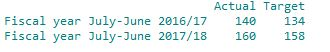
\includegraphics{Images/matrix.JPG}
\end{frame}


\begin{frame}[fragile]{Other examples}
\protect\hypertarget{other-examples}{}

\begin{Shaded}
\begin{Highlighting}[]
\NormalTok{A <-}\StringTok{ }\KeywordTok{matrix}\NormalTok{(}\KeywordTok{c}\NormalTok{(}\DecValTok{1}\NormalTok{, }\DecValTok{3}\NormalTok{, }\DecValTok{5}\NormalTok{, }\DecValTok{7}\NormalTok{, }\DecValTok{9}\NormalTok{, }\DecValTok{11}\NormalTok{, }\DecValTok{13}\NormalTok{, }\DecValTok{15}\NormalTok{, }\DecValTok{17}\NormalTok{),}
  \DataTypeTok{ncol =} \DecValTok{3}\NormalTok{,}
  \DataTypeTok{byrow =}\NormalTok{ F}
\NormalTok{)}
\NormalTok{A}
\end{Highlighting}
\end{Shaded}

\begin{verbatim}
##      [,1] [,2] [,3]
## [1,]    1    7   13
## [2,]    3    9   15
## [3,]    5   11   17
\end{verbatim}

\end{frame}

\begin{frame}[fragile]{}
\protect\hypertarget{section}{}

\begin{Shaded}
\begin{Highlighting}[]
\NormalTok{B <-}\StringTok{ }\KeywordTok{matrix}\NormalTok{(}\KeywordTok{c}\NormalTok{(}\DecValTok{2}\NormalTok{, }\DecValTok{4}\NormalTok{, }\DecValTok{6}\NormalTok{, }\DecValTok{8}\NormalTok{, }\DecValTok{10}\NormalTok{, }\DecValTok{12}\NormalTok{, }\DecValTok{14}\NormalTok{, }\DecValTok{16}\NormalTok{, }\DecValTok{18}\NormalTok{),}
  \DataTypeTok{ncol =} \DecValTok{3}\NormalTok{,}
  \DataTypeTok{byrow =}\NormalTok{ F}
\NormalTok{)}
\NormalTok{B}
\end{Highlighting}
\end{Shaded}

\begin{verbatim}
##      [,1] [,2] [,3]
## [1,]    2    8   14
## [2,]    4   10   16
## [3,]    6   12   18
\end{verbatim}

\end{frame}

\begin{frame}[fragile]{Matrices selection}
\protect\hypertarget{matrices-selection}{}

To select elements in a matrix we can use square brackets {[} , {]},
between the square brackets, you indicate the position of the row and
column in which the elements to select are.

To select the element in the first row and second column of matrix
\textbf{A}, you type \textbf{A}{[}1,2{]}.

To select the element in the third row and second column of matrix
\textbf{A}, you type \textbf{A}{[}3,2{]}, etc.

\begin{block}{Example}

\begin{Shaded}
\begin{Highlighting}[]
\NormalTok{A}
\NormalTok{A[}\DecValTok{1}\NormalTok{, }\DecValTok{2}\NormalTok{]}
\NormalTok{A[}\DecValTok{3}\NormalTok{, }\DecValTok{2}\NormalTok{]}
\end{Highlighting}
\end{Shaded}

\end{block}

\end{frame}

\begin{frame}[fragile]{Arithmetic Operation}
\protect\hypertarget{arithmetic-operation}{}

We can perform all the arithmetic operations on matrices

\begin{itemize}
\tightlist
\item
  Addition
\end{itemize}

\begin{Shaded}
\begin{Highlighting}[]
\NormalTok{C <-}\StringTok{ }\NormalTok{A }\OperatorTok{+}\StringTok{ }\NormalTok{B}
\NormalTok{C}
\end{Highlighting}
\end{Shaded}

\begin{verbatim}
##      [,1] [,2] [,3]
## [1,]    3   15   27
## [2,]    7   19   31
## [3,]   11   23   35
\end{verbatim}

\begin{itemize}
\tightlist
\item
  Subtraction
\end{itemize}

\begin{Shaded}
\begin{Highlighting}[]
\NormalTok{D <-}\StringTok{ }\NormalTok{B }\OperatorTok{-}\StringTok{ }\NormalTok{A}
\NormalTok{D}
\end{Highlighting}
\end{Shaded}

\begin{verbatim}
##      [,1] [,2] [,3]
## [1,]    1    1    1
## [2,]    1    1    1
## [3,]    1    1    1
\end{verbatim}

\end{frame}

\begin{frame}[fragile]{Arithmetic Operation}
\protect\hypertarget{arithmetic-operation-1}{}

\begin{block}{Multiplication}

\begin{Shaded}
\begin{Highlighting}[]
\NormalTok{F <-}\StringTok{ }\NormalTok{A }\OperatorTok\StringTok{ }\NormalTok{B}
\NormalTok{F}
\end{Highlighting}
\end{Shaded}

\begin{verbatim}
##      [,1] [,2] [,3]
## [1,]  108  234  360
## [2,]  132  294  456
## [3,]  156  354  552
\end{verbatim}

\end{block}

\end{frame}

\begin{frame}[fragile]{Arithmetic Operation}
\protect\hypertarget{arithmetic-operation-2}{}

\begin{itemize}
\tightlist
\item
  Transpose
\end{itemize}

\begin{align*}
G=t(A)=\begin{pmatrix}
1&7&13\\
3&9&15\\
5&11&17
\end{pmatrix}\end{align*}

\begin{Shaded}
\begin{Highlighting}[]
\NormalTok{G <-}\StringTok{ }\KeywordTok{t}\NormalTok{(A)}
\NormalTok{G}
\end{Highlighting}
\end{Shaded}

\begin{verbatim}
##      [,1] [,2] [,3]
## [1,]    1    3    5
## [2,]    7    9   11
## [3,]   13   15   17
\end{verbatim}

\end{frame}

\begin{frame}[fragile]{Arithmetic Operation}
\protect\hypertarget{arithmetic-operation-3}{}

\begin{itemize}
\tightlist
\item
  Determinant
\end{itemize}

\begin{align*}
G=det(A)=\begin{vmatrix}
1&7&13\\
3&9&15\\
5&11&17
\end{vmatrix}\end{align*}

\begin{Shaded}
\begin{Highlighting}[]
\NormalTok{G <-}\StringTok{ }\KeywordTok{det}\NormalTok{(A)}
\NormalTok{G}
\end{Highlighting}
\end{Shaded}

\begin{verbatim}
## [1] 4.263256e-14
\end{verbatim}

\end{frame}


\subsection{Dataframe}
\begin{frame}[fragile]{Dataframe}
\protect\hypertarget{dataframe}{}

Dataframes are another way to put data in tables! Unlike matrices,
dataframes can have different types of data!

A dataframe has the variables of a data set as \texttt{columns} and the
observations as \texttt{rows}. This will be a familiar concept for those
coming from different statistical software packages such as
\texttt{Excel}, \texttt{SPSS}, or \texttt{STATA}

The function for dataframe is \texttt{data.frame()}.

\end{frame}

\begin{frame}[fragile]{Example}
\protect\hypertarget{example-7}{}

\begin{Shaded}
\begin{Highlighting}[]
\CommentTok{# Make a dataframe with columns named a and b}
\KeywordTok{data.frame}\NormalTok{(}\DataTypeTok{a =} \DecValTok{2}\OperatorTok{:}\DecValTok{4}\NormalTok{, }\DataTypeTok{b =} \DecValTok{5}\OperatorTok{:}\DecValTok{7}\NormalTok{)}
\end{Highlighting}
\end{Shaded}

\begin{longtable}[]{@{}rr@{}}
\toprule
a & b\tabularnewline
\midrule
\endhead
2 & 5\tabularnewline
3 & 6\tabularnewline
4 & 7\tabularnewline
\bottomrule
\end{longtable}

The numbers \texttt{1\ 2\ 3} at the left on your \texttt{console} are
\texttt{row} labels and are not a \texttt{column} of the dataframe

Each column in a dataframe is a vector!

\end{frame}

\begin{frame}[fragile]{Dataframe}
\protect\hypertarget{dataframe-1}{}

\begin{block}{Example}

a \textless- c(6, 5, 1)

b \textless- c(1, 1, 3)

data \textless- data.frame(a, b) \texttt{\#} The output is ?

\end{block}

\begin{block}{Group work}

Create a dataframe and call it \texttt{data} for the following vectors:

\begin{Shaded}
\begin{Highlighting}[]
\CommentTok{# Set the same seed to get the same sample}
\KeywordTok{set.seed}\NormalTok{(}\DecValTok{123}\NormalTok{)}
\NormalTok{height <-}\StringTok{ }\KeywordTok{rnorm}\NormalTok{(}\DataTypeTok{n =} \DecValTok{100}\NormalTok{, }\DataTypeTok{mean =} \DecValTok{135}\NormalTok{, }\DataTypeTok{sd =} \DecValTok{12}\NormalTok{)}
\NormalTok{weight <-}\StringTok{ }\KeywordTok{rnorm}\NormalTok{(}\DataTypeTok{n =} \DecValTok{100}\NormalTok{, }\DataTypeTok{mean =} \DecValTok{55}\NormalTok{, }\DataTypeTok{sd =} \DecValTok{9}\NormalTok{)}
\end{Highlighting}
\end{Shaded}

\end{block}

\end{frame}

\begin{frame}[fragile]{Quick, have a look at your dataset}
\protect\hypertarget{quick-have-a-look-at-your-dataset}{}

Working with large datasets is common in data science. When you work
with (extremely) large datasets and dataframes, your first task as a
data analyst is to develop a clear understanding of its structure and
main elements. Therefore, it is often useful to show only part of the
entire dataset.

\begin{enumerate}
\item
  \texttt{head()}: enables you to show the first observations of a
  dataframe.
\item
  \texttt{tail()}: enables you to print out the last observations in
  your dataset.
\end{enumerate}

Both \texttt{head()} and \texttt{tail()} print a top line called
\texttt{header}, which contains the names of the different variables in
your data set.

\end{frame}

\begin{frame}[fragile]{Have a look at the structure}
\protect\hypertarget{have-a-look-at-the-structure}{}

Another method that is often used to get a rapid overview of your
dataset is the function \texttt{str()}.

\begin{enumerate}
\setcounter{enumi}{2}
\tightlist
\item
  \texttt{str()}: Shows you the structure of your dataset
\end{enumerate}

The structure of a dataframe tells you :

\begin{enumerate}
\tightlist
\item
  The total number of observations
\item
  The total number of variables
\item
  A full list of the variables names
\item
  The first observations
\end{enumerate}

\begin{block}{Note}

Applying the \texttt{str()} function will often be the first thing that
you do when receiving a new dataset or dataframe. It is a great way to
get more insight in your dataset before diving into the real analysis.

\end{block}

\end{frame}

\begin{frame}[fragile]{Example}
\protect\hypertarget{example-9}{}

Considering these vectors:


%%%%%%%%%%%%%%%

\begin{Shaded}
\begin{Highlighting}[]
\CommentTok{# Set the same seed to get the same sample}
\KeywordTok{set.seed}\NormalTok{(}\DecValTok{123}\NormalTok{)}
\NormalTok{height <-}\StringTok{ }\KeywordTok{rnorm}\NormalTok{(}\DataTypeTok{n =} \DecValTok{100}\NormalTok{, }\DataTypeTok{mean =} \DecValTok{155}\NormalTok{, }\DataTypeTok{sd =} \DecValTok{13}\NormalTok{)}
\NormalTok{weight <-}\StringTok{ }\KeywordTok{rnorm}\NormalTok{(}\DataTypeTok{n =} \DecValTok{100}\NormalTok{, }\DataTypeTok{mean =} \DecValTok{69}\NormalTok{, }\DataTypeTok{sd =} \DecValTok{11}\NormalTok{)}
\end{Highlighting}
	\end{Shaded}
	
Create a \texttt{dataframe} for it.

\begin{Shaded}
\begin{Highlighting}[]
\NormalTok{data <-}\StringTok{ }\KeywordTok{data.frame}\NormalTok{(height, weight)}
\end{Highlighting}
\end{Shaded}

\begin{Shaded}
\begin{Highlighting}[]
\KeywordTok{str}\NormalTok{(data)}
\end{Highlighting}
\end{Shaded}

\begin{verbatim}
## 'data.frame':    120 obs. of  2 variables:
##  $ height: num  161 150 131 141 130 129 125 127 154 134 ...
##  $ weight: num  58 66 43 61 51 62 55 61 68 56 ...
\end{verbatim}

\end{frame}

\begin{frame}[fragile]{Example}
\protect\hypertarget{example-10}{}

\begin{Shaded}
\begin{Highlighting}[]
\KeywordTok{head}\NormalTok{(data, }\DecValTok{5}\NormalTok{)}
\end{Highlighting}
\end{Shaded}

\begin{longtable}[]{@{}rr@{}}
\toprule
height & weight\tabularnewline
\midrule
\endhead
161 & 58\tabularnewline
150 & 66\tabularnewline
131 & 43\tabularnewline
141 & 61\tabularnewline
130 & 51\tabularnewline
\bottomrule
\end{longtable}

\begin{Shaded}
\begin{Highlighting}[]
\KeywordTok{tail}\NormalTok{(data, }\DecValTok{3}\NormalTok{)}
\end{Highlighting}
\end{Shaded}

\begin{longtable}[]{@{}lrr@{}}
\toprule
& height & weight\tabularnewline
\midrule
\endhead
118 & 119 & 65\tabularnewline
119 & 155 & 35\tabularnewline
120 & 145 & 67\tabularnewline
\bottomrule
\end{longtable}

\end{frame}

\begin{frame}[fragile]{Using built-in datasets in R}
\protect\hypertarget{using-built-in-datasets-in-r}{}

There are several ways to find the included datasets in R.

Using \texttt{data()} will give you a list of the datasets of all loaded
packages.

\begin{block}{Example}

\texttt{\#} This shows all the R datasets in the package
\texttt{datasets}.

data()

\end{block}

\begin{block}{Example}

library(datasets)

data \textless- airquality

str(data)

To get help in the proper description of the dataset
\texttt{?airquality}

\end{block}

\end{frame}

\begin{frame}{The end}
\protect\hypertarget{the-end}{}

\begin{center}
\textbf{Thank you!}
\end{center}

\end{frame}

\begin{frame}{References}
\protect\hypertarget{references}{}

\begin{thebibliography}{99}
\bibitem {P} 
Wickham, H., \& Grolemund, G. (2016). R for data science: import, tidy, transform, visualize, and model data. " O'Reilly Media, Inc.".
\end{thebibliography}

\end{frame}

\end{document}
